% Options for packages loaded elsewhere
\PassOptionsToPackage{unicode}{hyperref}
\PassOptionsToPackage{hyphens}{url}
\PassOptionsToPackage{dvipsnames,svgnames,x11names}{xcolor}
%
\documentclass[
]{report}

\usepackage{amsmath,amssymb}
\usepackage{iftex}
\ifPDFTeX
  \usepackage[T1]{fontenc}
  \usepackage[utf8]{inputenc}
  \usepackage{textcomp} % provide euro and other symbols
\else % if luatex or xetex
  \usepackage{unicode-math}
  \defaultfontfeatures{Scale=MatchLowercase}
  \defaultfontfeatures[\rmfamily]{Ligatures=TeX,Scale=1}
\fi
\usepackage{lmodern}
\ifPDFTeX\else  
    % xetex/luatex font selection
\fi
% Use upquote if available, for straight quotes in verbatim environments
\IfFileExists{upquote.sty}{\usepackage{upquote}}{}
\IfFileExists{microtype.sty}{% use microtype if available
  \usepackage[]{microtype}
  \UseMicrotypeSet[protrusion]{basicmath} % disable protrusion for tt fonts
}{}
\makeatletter
\@ifundefined{KOMAClassName}{% if non-KOMA class
  \IfFileExists{parskip.sty}{%
    \usepackage{parskip}
  }{% else
    \setlength{\parindent}{0pt}
    \setlength{\parskip}{6pt plus 2pt minus 1pt}}
}{% if KOMA class
  \KOMAoptions{parskip=half}}
\makeatother
\usepackage{xcolor}
\usepackage[left = 20.0mm,right = 20.0mm,marginparsep =
7.7mm,marginparwidth = 70.3mm,top = 20mm]{geometry}
\setlength{\emergencystretch}{3em} % prevent overfull lines
\setcounter{secnumdepth}{5}
% Make \paragraph and \subparagraph free-standing
\makeatletter
\ifx\paragraph\undefined\else
  \let\oldparagraph\paragraph
  \renewcommand{\paragraph}{
    \@ifstar
      \xxxParagraphStar
      \xxxParagraphNoStar
  }
  \newcommand{\xxxParagraphStar}[1]{\oldparagraph*{#1}\mbox{}}
  \newcommand{\xxxParagraphNoStar}[1]{\oldparagraph{#1}\mbox{}}
\fi
\ifx\subparagraph\undefined\else
  \let\oldsubparagraph\subparagraph
  \renewcommand{\subparagraph}{
    \@ifstar
      \xxxSubParagraphStar
      \xxxSubParagraphNoStar
  }
  \newcommand{\xxxSubParagraphStar}[1]{\oldsubparagraph*{#1}\mbox{}}
  \newcommand{\xxxSubParagraphNoStar}[1]{\oldsubparagraph{#1}\mbox{}}
\fi
\makeatother

\usepackage{color}
\usepackage{fancyvrb}
\newcommand{\VerbBar}{|}
\newcommand{\VERB}{\Verb[commandchars=\\\{\}]}
\DefineVerbatimEnvironment{Highlighting}{Verbatim}{commandchars=\\\{\}}
% Add ',fontsize=\small' for more characters per line
\usepackage{framed}
\definecolor{shadecolor}{RGB}{241,243,245}
\newenvironment{Shaded}{\begin{snugshade}}{\end{snugshade}}
\newcommand{\AlertTok}[1]{\textcolor[rgb]{0.68,0.00,0.00}{#1}}
\newcommand{\AnnotationTok}[1]{\textcolor[rgb]{0.37,0.37,0.37}{#1}}
\newcommand{\AttributeTok}[1]{\textcolor[rgb]{0.40,0.45,0.13}{#1}}
\newcommand{\BaseNTok}[1]{\textcolor[rgb]{0.68,0.00,0.00}{#1}}
\newcommand{\BuiltInTok}[1]{\textcolor[rgb]{0.00,0.23,0.31}{#1}}
\newcommand{\CharTok}[1]{\textcolor[rgb]{0.13,0.47,0.30}{#1}}
\newcommand{\CommentTok}[1]{\textcolor[rgb]{0.37,0.37,0.37}{#1}}
\newcommand{\CommentVarTok}[1]{\textcolor[rgb]{0.37,0.37,0.37}{\textit{#1}}}
\newcommand{\ConstantTok}[1]{\textcolor[rgb]{0.56,0.35,0.01}{#1}}
\newcommand{\ControlFlowTok}[1]{\textcolor[rgb]{0.00,0.23,0.31}{\textbf{#1}}}
\newcommand{\DataTypeTok}[1]{\textcolor[rgb]{0.68,0.00,0.00}{#1}}
\newcommand{\DecValTok}[1]{\textcolor[rgb]{0.68,0.00,0.00}{#1}}
\newcommand{\DocumentationTok}[1]{\textcolor[rgb]{0.37,0.37,0.37}{\textit{#1}}}
\newcommand{\ErrorTok}[1]{\textcolor[rgb]{0.68,0.00,0.00}{#1}}
\newcommand{\ExtensionTok}[1]{\textcolor[rgb]{0.00,0.23,0.31}{#1}}
\newcommand{\FloatTok}[1]{\textcolor[rgb]{0.68,0.00,0.00}{#1}}
\newcommand{\FunctionTok}[1]{\textcolor[rgb]{0.28,0.35,0.67}{#1}}
\newcommand{\ImportTok}[1]{\textcolor[rgb]{0.00,0.46,0.62}{#1}}
\newcommand{\InformationTok}[1]{\textcolor[rgb]{0.37,0.37,0.37}{#1}}
\newcommand{\KeywordTok}[1]{\textcolor[rgb]{0.00,0.23,0.31}{\textbf{#1}}}
\newcommand{\NormalTok}[1]{\textcolor[rgb]{0.00,0.23,0.31}{#1}}
\newcommand{\OperatorTok}[1]{\textcolor[rgb]{0.37,0.37,0.37}{#1}}
\newcommand{\OtherTok}[1]{\textcolor[rgb]{0.00,0.23,0.31}{#1}}
\newcommand{\PreprocessorTok}[1]{\textcolor[rgb]{0.68,0.00,0.00}{#1}}
\newcommand{\RegionMarkerTok}[1]{\textcolor[rgb]{0.00,0.23,0.31}{#1}}
\newcommand{\SpecialCharTok}[1]{\textcolor[rgb]{0.37,0.37,0.37}{#1}}
\newcommand{\SpecialStringTok}[1]{\textcolor[rgb]{0.13,0.47,0.30}{#1}}
\newcommand{\StringTok}[1]{\textcolor[rgb]{0.13,0.47,0.30}{#1}}
\newcommand{\VariableTok}[1]{\textcolor[rgb]{0.07,0.07,0.07}{#1}}
\newcommand{\VerbatimStringTok}[1]{\textcolor[rgb]{0.13,0.47,0.30}{#1}}
\newcommand{\WarningTok}[1]{\textcolor[rgb]{0.37,0.37,0.37}{\textit{#1}}}

\providecommand{\tightlist}{%
  \setlength{\itemsep}{0pt}\setlength{\parskip}{0pt}}\usepackage{longtable,booktabs,array}
\usepackage{calc} % for calculating minipage widths
% Correct order of tables after \paragraph or \subparagraph
\usepackage{etoolbox}
\makeatletter
\patchcmd\longtable{\par}{\if@noskipsec\mbox{}\fi\par}{}{}
\makeatother
% Allow footnotes in longtable head/foot
\IfFileExists{footnotehyper.sty}{\usepackage{footnotehyper}}{\usepackage{footnote}}
\makesavenoteenv{longtable}
\usepackage{graphicx}
\makeatletter
\newsavebox\pandoc@box
\newcommand*\pandocbounded[1]{% scales image to fit in text height/width
  \sbox\pandoc@box{#1}%
  \Gscale@div\@tempa{\textheight}{\dimexpr\ht\pandoc@box+\dp\pandoc@box\relax}%
  \Gscale@div\@tempb{\linewidth}{\wd\pandoc@box}%
  \ifdim\@tempb\p@<\@tempa\p@\let\@tempa\@tempb\fi% select the smaller of both
  \ifdim\@tempa\p@<\p@\scalebox{\@tempa}{\usebox\pandoc@box}%
  \else\usebox{\pandoc@box}%
  \fi%
}
% Set default figure placement to htbp
\def\fps@figure{htbp}
\makeatother

\makeatletter
\@ifpackageloaded{caption}{}{\usepackage{caption}}
\AtBeginDocument{%
\ifdefined\contentsname
  \renewcommand*\contentsname{Table of contents}
\else
  \newcommand\contentsname{Table of contents}
\fi
\ifdefined\listfigurename
  \renewcommand*\listfigurename{List of Figures}
\else
  \newcommand\listfigurename{List of Figures}
\fi
\ifdefined\listtablename
  \renewcommand*\listtablename{List of Tables}
\else
  \newcommand\listtablename{List of Tables}
\fi
\ifdefined\figurename
  \renewcommand*\figurename{Figure}
\else
  \newcommand\figurename{Figure}
\fi
\ifdefined\tablename
  \renewcommand*\tablename{Table}
\else
  \newcommand\tablename{Table}
\fi
}
\@ifpackageloaded{float}{}{\usepackage{float}}
\floatstyle{ruled}
\@ifundefined{c@chapter}{\newfloat{codelisting}{h}{lop}}{\newfloat{codelisting}{h}{lop}[chapter]}
\floatname{codelisting}{Listing}
\newcommand*\listoflistings{\listof{codelisting}{List of Listings}}
\makeatother
\makeatletter
\makeatother
\makeatletter
\@ifpackageloaded{caption}{}{\usepackage{caption}}
\@ifpackageloaded{subcaption}{}{\usepackage{subcaption}}
\makeatother
\makeatletter
\@ifpackageloaded{tcolorbox}{}{\usepackage[skins,breakable]{tcolorbox}}
\makeatother
\makeatletter
\@ifundefined{shadecolor}{\definecolor{shadecolor}{rgb}{.97, .97, .97}}{}
\makeatother
\makeatletter
\@ifundefined{codebgcolor}{\definecolor{codebgcolor}{HTML}{EEEEEE}}{}
\makeatother
\makeatletter
\ifdefined\Shaded\renewenvironment{Shaded}{\begin{tcolorbox}[enhanced, colback={codebgcolor}, breakable, frame hidden, boxrule=0pt, sharp corners]}{\end{tcolorbox}}\fi
\makeatother

\usepackage{bookmark}

\IfFileExists{xurl.sty}{\usepackage{xurl}}{} % add URL line breaks if available
\urlstyle{same} % disable monospaced font for URLs
\hypersetup{
  pdftitle={Efficient Filtering and Fitting of Models Derived from Integro-Difference Equations},
  pdfauthor={Evan Tate Paterson Hughes},
  colorlinks=true,
  linkcolor={blue},
  filecolor={Maroon},
  citecolor={Blue},
  urlcolor={Blue},
  pdfcreator={LaTeX via pandoc}}


\title{Efficient Filtering and Fitting of Models Derived from
Integro-Difference Equations}
\author{Evan Tate Paterson Hughes}
\date{}

\begin{document}
\maketitle

\renewcommand*\contentsname{Table of contents}
{
\hypersetup{linkcolor=}
\setcounter{tocdepth}{2}
\tableofcontents
}

: : : \{.content-visible unless-format = ``pdf''\}
\href{../index.html}{Index} : : :

\begin{verbatim}
# Fitting IDEM using ```jax_idem```
\end{verbatim}

The primary use of the jax\_idem package is to fit Integro-difference
equation models to data.

Currently, the only supported way to do this is through
maximum-likelihood estimation with the kalman/information filter and
OPTAX.

\chapter{Simple example; synthetic simple
data}\label{simple-example-synthetic-simple-data}

We will start by simulating from a simple IDEM with only three time
steps. We can quickly make a model using \texttt{gen\_example\_idem}

\begin{Shaded}
\begin{Highlighting}[]
\ImportTok{import}\NormalTok{ jax}
\ImportTok{import}\NormalTok{ jax.random }\ImportTok{as}\NormalTok{ rand}
\ImportTok{import}\NormalTok{ jax.numpy }\ImportTok{as}\NormalTok{ jnp}

\NormalTok{jax.config.update(}\StringTok{\textquotesingle{}jax\_enable\_x64\textquotesingle{}}\NormalTok{, }\VariableTok{False}\NormalTok{)}

\ImportTok{import}\NormalTok{ matplotlib.pyplot }\ImportTok{as}\NormalTok{ plt}

\ImportTok{import}\NormalTok{ sys}
\ImportTok{import}\NormalTok{ os}
\NormalTok{sys.path.append(os.path.abspath(}\StringTok{\textquotesingle{}../src/jaxidem\textquotesingle{}}\NormalTok{))}
\ImportTok{import}\NormalTok{ idem}
\ImportTok{import}\NormalTok{ utilities}
\ImportTok{import}\NormalTok{ filter\_smoother\_functions }\ImportTok{as}\NormalTok{ fsf}

\ImportTok{import}\NormalTok{ importlib}
\NormalTok{importlib.}\BuiltInTok{reload}\NormalTok{(idem)}
\NormalTok{importlib.}\BuiltInTok{reload}\NormalTok{(utilities)}
\NormalTok{importlib.}\BuiltInTok{reload}\NormalTok{(fsf)}
\end{Highlighting}
\end{Shaded}

\begin{Shaded}
\begin{Highlighting}[]
\NormalTok{key }\OperatorTok{=}\NormalTok{ jax.random.PRNGKey(}\DecValTok{1}\NormalTok{)}
\NormalTok{keys }\OperatorTok{=}\NormalTok{ rand.split(key, }\DecValTok{3}\NormalTok{)}

\NormalTok{process\_basis }\OperatorTok{=}\NormalTok{ utilities.place\_basis(nres}\OperatorTok{=}\DecValTok{1}\NormalTok{, min\_knot\_num}\OperatorTok{=}\DecValTok{5}\NormalTok{)}
\NormalTok{nbasis }\OperatorTok{=}\NormalTok{ process\_basis.nbasis}

\NormalTok{m\_0 }\OperatorTok{=}\NormalTok{ jnp.zeros(nbasis).at[}\DecValTok{20}\NormalTok{].}\BuiltInTok{set}\NormalTok{(}\DecValTok{10}\NormalTok{)}
\NormalTok{sigma2\_0 }\OperatorTok{=} \FloatTok{0.0001}

\NormalTok{truemodel }\OperatorTok{=}\NormalTok{ idem.gen\_example\_idem(}
\NormalTok{    keys[}\DecValTok{0}\NormalTok{], k\_spat\_inv}\OperatorTok{=}\VariableTok{True}\NormalTok{,}
\NormalTok{    process\_basis}\OperatorTok{=}\NormalTok{process\_basis,}
\NormalTok{    m\_0}\OperatorTok{=}\NormalTok{m\_0, sigma2\_0}\OperatorTok{=}\NormalTok{sigma2\_0,}
\NormalTok{    sigma2\_eta}\OperatorTok{=}\FloatTok{0.02}\OperatorTok{**}\DecValTok{2}\NormalTok{,}
\NormalTok{    sigma2\_eps}\OperatorTok{=}\FloatTok{0.05}\OperatorTok{**}\DecValTok{2}
\NormalTok{)}

\NormalTok{process\_data, obs\_data }\OperatorTok{=}\NormalTok{ truemodel.simulate(nobs}\OperatorTok{=}\DecValTok{50}\NormalTok{, T}\OperatorTok{=}\DecValTok{3}\NormalTok{, key}\OperatorTok{=}\NormalTok{keys[}\DecValTok{1}\NormalTok{])}

\NormalTok{process\_data.save\_plot(}\StringTok{"true\_process.png"}\NormalTok{)}
\NormalTok{obs\_data.save\_plot(}\StringTok{"synthetic\_data.png"}\NormalTok{)}
\end{Highlighting}
\end{Shaded}

\begin{figure}

\centering{

\begin{figure}
\centering
\pandocbounded{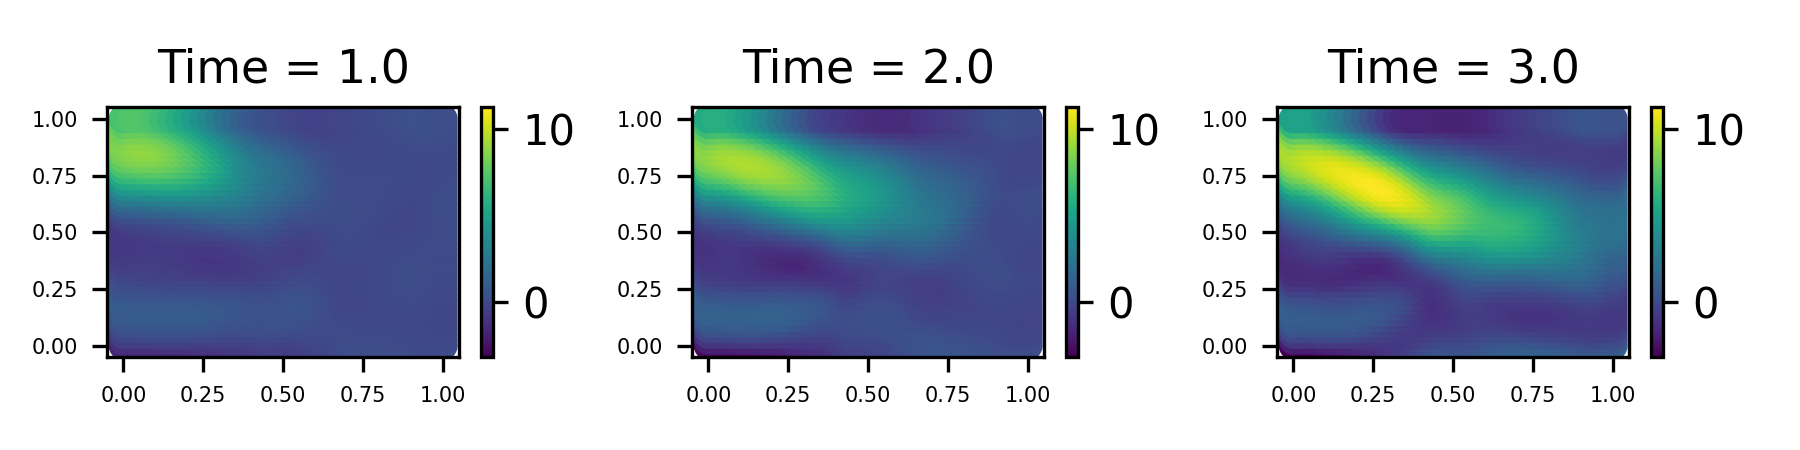
\includegraphics[keepaspectratio]{true_process.png}}
\caption{Process}
\end{figure}

\begin{figure}
\centering
\pandocbounded{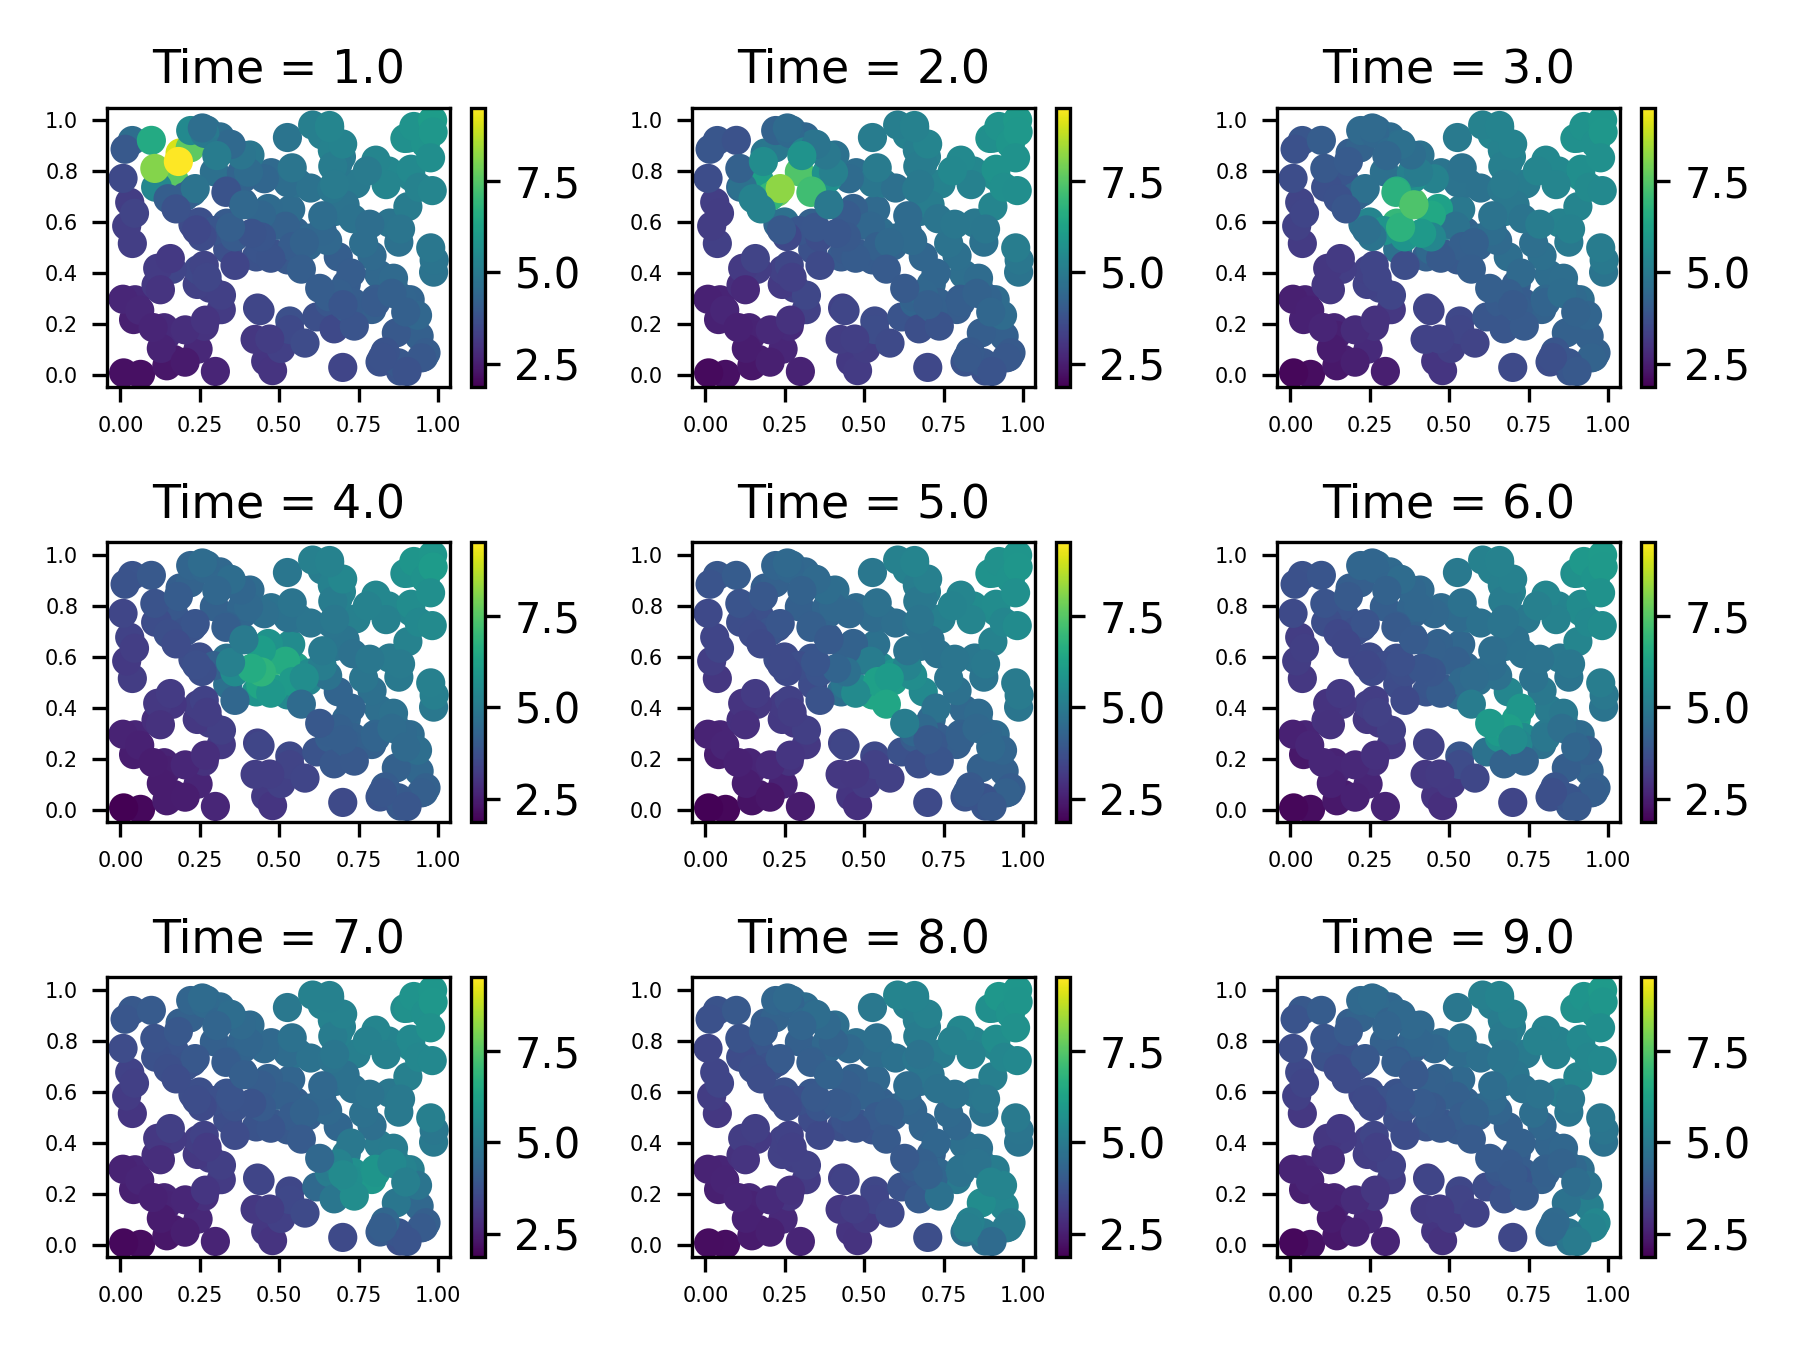
\includegraphics[keepaspectratio]{synthetic_data.png}}
\caption{Observations}
\end{figure}

}

\caption{\label{fig-example}An example target simulation, with the
underlying process (left), and noisy observations (right).}

\end{figure}%

Note that there is one missing process time point that is not plotted
here; \(t=0\). In the version of the model used, data is only taken at
\(t=1,2,3\), while it is assumed that the process exists from time 0.

\section{Fitting}\label{fitting}

Now, after we initialise with a `guess' baseline model, we can use
\texttt{idem.IDEM\_model.fit\_kalman\_filter} (recomended for fixed data
observation locations) or \texttt{fit\_information\_filter} to fit the
model to the synthetic data.

\begin{Shaded}
\begin{Highlighting}[]
\NormalTok{K\_basis }\OperatorTok{=}\NormalTok{ truemodel.kernel.basis}
\CommentTok{\# scale and shape of the kernel will be the same, but the offsets will be estimated}
\NormalTok{k }\OperatorTok{=}\NormalTok{ (}
\NormalTok{    jnp.array([}\FloatTok{200.0}\NormalTok{]),}
\NormalTok{    jnp.array([}\FloatTok{0.001}\NormalTok{]),}
\NormalTok{    jnp.array([}\FloatTok{0.0}\NormalTok{]),}
\NormalTok{    jnp.array([}\FloatTok{0.0}\NormalTok{]),}
\NormalTok{)}
\CommentTok{\# This is the kind of kernel used by \textasciigrave{}\textasciigrave{}\textasciigrave{}gen\_example\_idem\textasciigrave{}\textasciigrave{}\textasciigrave{}}
\NormalTok{kernel }\OperatorTok{=}\NormalTok{ idem.param\_exp\_kernel(K\_basis, k)}

\NormalTok{model0 }\OperatorTok{=}\NormalTok{ idem.IDEM\_Model(}
\NormalTok{                    process\_basis }\OperatorTok{=}\NormalTok{ process\_basis,}
\NormalTok{                    kernel}\OperatorTok{=}\NormalTok{kernel,}
\NormalTok{                    process\_grid }\OperatorTok{=}\NormalTok{ utilities.create\_grid(jnp.array([[}\DecValTok{0}\NormalTok{, }\DecValTok{1}\NormalTok{], [}\DecValTok{0}\NormalTok{, }\DecValTok{1}\NormalTok{]]),}
\NormalTok{                                               jnp.array([}\DecValTok{41}\NormalTok{, }\DecValTok{41}\NormalTok{])),}
\NormalTok{                    sigma2\_eta }\OperatorTok{=} \FloatTok{0.01}\OperatorTok{**}\DecValTok{2}\NormalTok{,}
\NormalTok{                    sigma2\_eps }\OperatorTok{=} \FloatTok{0.01}\OperatorTok{**}\DecValTok{2}\NormalTok{,}
\NormalTok{                    beta }\OperatorTok{=}\NormalTok{ jnp.array([}\FloatTok{0.0}\NormalTok{, }\FloatTok{0.0}\NormalTok{, }\FloatTok{0.0}\NormalTok{]),}
\NormalTok{                    m\_0 }\OperatorTok{=}\NormalTok{ jnp.zeros(nbasis),}
\NormalTok{                    sigma2\_0}\OperatorTok{=}\DecValTok{10}\OperatorTok{*}\NormalTok{jnp.eye(nbasis))}
\end{Highlighting}
\end{Shaded}

For context, the true values of the kernel parameters are

\begin{Shaded}
\begin{Highlighting}[]
\BuiltInTok{print}\NormalTok{(truemodel.kernel.params)}
\end{Highlighting}
\end{Shaded}

\begin{verbatim}
(Array([150.], dtype=float32), Array([0.002], dtype=float32), Array([-0.1], dtype=float32), Array([0.1], dtype=float32))
\end{verbatim}

So we've chosen a model with high prior variance and no flow, with
inaccurate guesses for the spread, diffusion, and variances.

The fitting functions output new \texttt{IDEM\_Model} objects, generated
using OPTAX to optimise for the likelihood.

\begin{Shaded}
\begin{Highlighting}[]
\NormalTok{obs\_data\_wide }\OperatorTok{=}\NormalTok{ obs\_data.as\_wide()}
\NormalTok{X\_obs }\OperatorTok{=}\NormalTok{ jnp.column\_stack([jnp.ones(obs\_data\_wide[}\StringTok{\textquotesingle{}x\textquotesingle{}}\NormalTok{].shape[}\DecValTok{0}\NormalTok{]), obs\_data\_wide[}\StringTok{\textquotesingle{}x\textquotesingle{}}\NormalTok{], obs\_data\_wide[}\StringTok{\textquotesingle{}y\textquotesingle{}}\NormalTok{]])}

\ImportTok{import}\NormalTok{ optax}
\NormalTok{model1 }\OperatorTok{=}\NormalTok{ model0.fit\_kalman\_filter(obs\_data}\OperatorTok{=}\NormalTok{obs\_data,}
\NormalTok{                                  X\_obs}\OperatorTok{=}\NormalTok{X\_obs,}
\NormalTok{                                  fixed\_ind}\OperatorTok{=}\NormalTok{[}\StringTok{"m\_0"}\NormalTok{, }\StringTok{"sigma2\_0"}\NormalTok{, }\StringTok{"beta"}\NormalTok{],}
\NormalTok{                                  nits}\OperatorTok{=}\DecValTok{100}\NormalTok{,}
\NormalTok{                                  optimizer}\OperatorTok{=}\NormalTok{optax.adam(}\FloatTok{1e{-}1}\NormalTok{),)}
\end{Highlighting}
\end{Shaded}

\begin{Shaded}
\begin{Highlighting}[]
\BuiltInTok{print}\NormalTok{(model1.kernel.params)}
\BuiltInTok{print}\NormalTok{(model1.sigma2\_eps, }\StringTok{"truth:"}\NormalTok{, }\FloatTok{0.05}\OperatorTok{**}\DecValTok{2}\NormalTok{)}
\BuiltInTok{print}\NormalTok{(model1.sigma2\_eta, }\StringTok{"truth:"}\NormalTok{, }\FloatTok{0.02}\OperatorTok{**}\DecValTok{2}\NormalTok{)}
\end{Highlighting}
\end{Shaded}

\begin{verbatim}
(Array([nan], dtype=float32), Array([nan], dtype=float32), Array([nan], dtype=float32), Array([nan], dtype=float32))
nan truth: 0.0025000000000000005
nan truth: 0.0004
\end{verbatim}




\end{document}
